\chapter{Dataset Analysis and Results}
\label{chap:results}

This chapter showcases what the scraper makes possible: it exercises the new collection layers on the corpus to show the kinds of analysis they open up, rather than presenting the dataset as a body of settled evidence. It is organised around the contributions claimed in the Introduction rather than around the data schema: each section delivers one of those contributions and traces it back to the collection mechanism that made it possible. Section~\ref{sec:res-corpus} characterises what the corpus actually is relative to other Telegram datasets, establishing the framing on which every later section rests. Section~\ref{sec:res-network} reconstructs the forward graph from the corpus and corrects several common misreadings of it. Section~\ref{sec:res-layers} is the core: it presents the three core capability layers (comments, edits, and deletions), of which edits and deletions are collected by no prior general-purpose Telegram corpus and comments only by the concurrent TeraGram~\cite{teragram2026}, together with per-platform restriction, a signal prior corpora left unexposed inside serialized message objects; it then gathers the supporting content layers (engagement, language, polls, and service actions) and a set of deliberate null results. Section~\ref{sec:res-war} exercises several of these layers at once on a single current-events showcase, the 2026 US/Israel--Iran war.

%======================================================================
\section{What the Corpus Is}
\label{sec:res-corpus}
%======================================================================

We crawled $12{,}065$ channels for messages, just $2.6\%$ of the $456{,}554$ channels the database registers. The crawled set is composed of a random subset of TGDataset's channels~\cite{lamorgia2025} plus their linked discussion groups where available; the remaining $97.4\%$ is a discovery frontier of channels that were referenced but never pulled (Section~\ref{sec:res-frontier}). The value of this dataset is therefore not breadth but \emph{per-channel depth}: the comments, edits, deletions, and metadata snapshots collected for the channels we did crawl. Table~\ref{tab:res-scalars} summarises the corpus and isolates the additive layers that distinguish it from prior work.

\begin{table}[htbp]
\centering
\caption[Corpus scalars and additive layers.]{Corpus scalars (top) and the additive layers it captures beyond the broadcast text (bottom). Counts are as of June~2026; the message total is the sum of the broadcast side ($141.8$\,M) and the linked-group discussion side ($333.2$\,M).}
\label{tab:res-scalars}
\small
\begin{tabular}{@{}lr@{}}
\toprule
\textbf{Quantity} & \textbf{Value} \\
\midrule
Messages (total)                    & $474.9$\,M \\
\quad broadcast side                & $141.8$\,M \\
\quad linked-group discussion side  & $333.2$\,M \\
Channels with collected messages    & $12{,}065$ \\
Registered channels (incl.\ frontier) & $456{,}554$ \\
Time span                           & Sep 2015 -- Jun 2026 \\
\midrule
\multicolumn{2}{@{}l}{\textit{Additive layers (beyond the broadcast text)}} \\
Linked-group comments / replies     & $333.2$\,M \\
Messages carrying reactions         & $116.8$\,M \\
Detected deletions                  & $2.42$\,M \\
Metadata snapshots                  & $37{,}669$ \\
Archived edits (with before/after text) & $36{,}016$ \\
Polls                               & $323{,}389$ \\
\bottomrule
\end{tabular}
\end{table}

\paragraph{Small by design.}
Set against public Telegram datasets (Tables~\ref{tab:dataset-comparison} and~\ref{tab:dataset-richness}), this corpus is deliberately small in channel count: its $8{,}284$ metadata-bearing broadcast channels sit far below the large general-purpose crawls, which reach hundreds of thousands of channels, and on the broadcast side ($141.8$\,M messages) it is a \emph{subset} of what they hold. It does not compete on breadth, and its contribution is orthogonal to size. Because every channel is revisited over time, the corpus records how content and channels \emph{change}, the message edits, deletions, and longitudinal metadata that no prior general-purpose corpus collected, and it captures the linked-group discussion side at full depth (the $333.2$\,M-message comment layer of Table~\ref{tab:res-scalars}, itself larger than the entire broadcast side). This deliberate trade, a smaller set of channels each revisited and captured in full rather than many channels sampled once, is the framing every downstream result depends on.

Of the $8{,}284$ broadcast channels that carry a metadata snapshot, $258$ ($3.1\%$) are verified, $8{,}021$ ($96.8\%$) are ordinary, and only five carry the scam flag.\footnote{Three of the five are impersonation personas tied to US far-right and QAnon content: a fake \emph{Politico} feed and accounts posing as Michael Flynn and Dan Scavino. The other two are a Russian crypto-investment fraud (fabricated deposit-to-profit screenshots) and a German Reichs\-b\"urger conspiracy channel that forwards heavily and links onward to successor channels to survive bans. All five were already inactive when flagged (their last posts fall in 2022--2024, against snapshots taken in 2026), and the flag is Telegram-assigned rather than scraper-derived: each carries Telegram's own injected warning string as its description.} The verified rate is roughly six times TGDataset's $0.54\%$.

\paragraph{Volume and depth in shape.}
Figure~\ref{fig:res-daily-messages} decomposes daily message volume into its two margins: total volume (top) is the number of channels active that day (middle, the extensive margin) times the mean messages per active channel that day (bottom, the intensive margin). The decomposition matters because the raw total cannot, on its own, separate genuine activity growth from the age composition of the sampled channels: most sampled channels were created and became active only later, so early dates are mechanically sparse regardless of underlying activity. Keeping in mind how dataset was seeded, almost all of the headline rise is the extensive margin: the active-channel count climbs by almost two orders of magnitude from 2016 into 2021, then plateaus near $5{,}500$--$6{,}000$ and edges down slightly thereafter, tracking when the sampled channels entered the corpus rather than any per-channel intensification. The intensive margin is far flatter: messages per active channel hold near $18$ from 2016 through 2019, then climb gradually to roughly $40$ by 2024 and $\sim 46$ by 2025, with sharp, short-lived spikes around major external events (Russia's 2022 invasion of Ukraine and the 2026 Maduro capture). The neutral reading therefore stands: the post-2022 concentration of volume is largely a composition and platform-growth effect rather than evidence that individual channels post dramatically more, though a modest genuine intensive rise and clear event-responsiveness are both visible in recent years. The per-channel depth distribution is shown in Figure~\ref{fig:res-channel-depth}: each channel's lifetime message total (not the daily intensive rate above) spans roughly five orders of magnitude, with most channels holding between $10^3$ and $10^4$ messages and a long upper tail reaching past $10^6$, so per-channel depth is dominated by a minority of very deep channels while the median channel is far shallower. Channel-class cumulative distributions confirm that the deepest channels are overwhelmingly the discussion groups, which is exactly where the comment layer lives.

\begin{figure}[htbp]
\centering
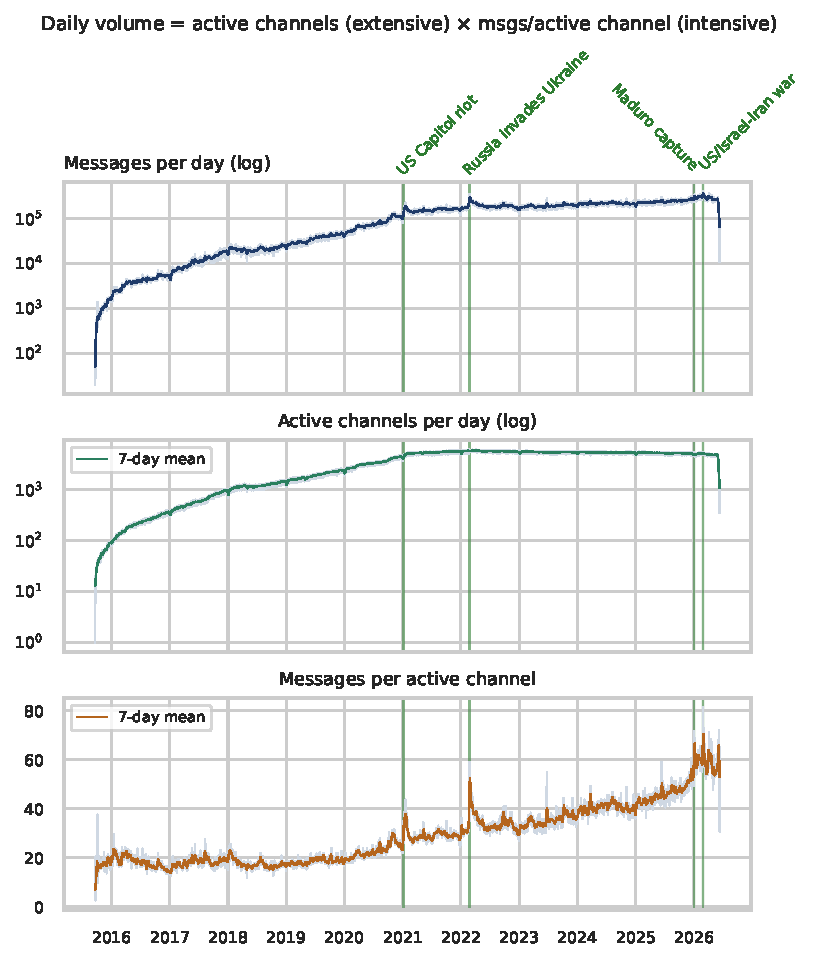
\includegraphics[width=\textwidth]{figures/res_daily_messages_normalised}
\caption[Daily message volume, decomposed.]{Daily message volume decomposed into extensive and intensive margins (Sep 2015 -- Jun 2026, $7$-day means; dashed lines mark external events). Top: total messages per day (log). Middle: number of channels active each day (log), the extensive margin. Bottom: mean messages per active channel each day, the intensive margin. The headline rise is almost entirely extensive (more channels active, saturating around 2021 as sampled channels enter the corpus); per-active-channel volume is far flatter, with only a modest recent rise and short event-driven spikes.}
\label{fig:res-daily-messages}
\end{figure}

\begin{figure}[htbp]
\centering
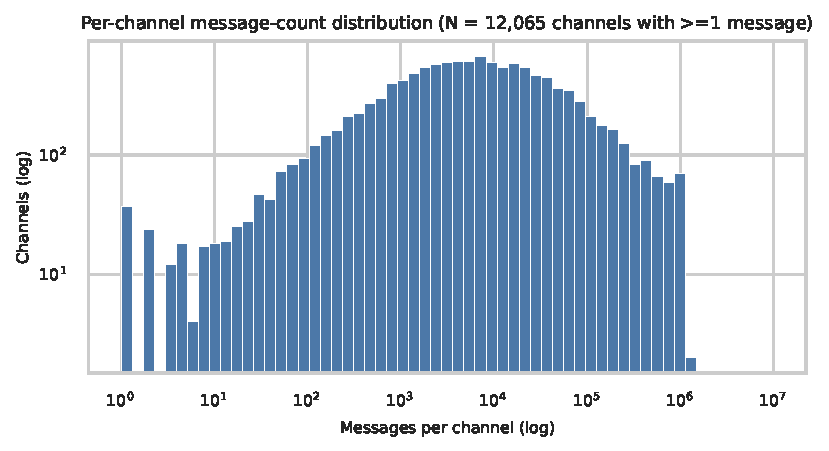
\includegraphics[width=\textwidth]{figures/res_channel_message_dist}
\caption[Per-channel message-count distribution.]{Distribution of per-channel lifetime message counts (log-binned, log--log axes). The distribution is unimodal: most of the $12{,}065$ crawled channels hold between $10^3$ and $10^4$ messages, with a long upper tail reaching past $10^6$. Depth spans several orders of magnitude, so the median channel is far shallower than the deepest, and a minority of very deep channels carries the corpus, which is why per-channel depth, not channel count, is the right scale on which to read this dataset.}
\label{fig:res-channel-depth}
\end{figure}

\paragraph{Posting follows a clear diurnal and weekly rhythm.}
The timing of posting characterises the active population as much as its size does. Figure~\ref{fig:res-activity-heatmap} aggregates message timestamps over the last twelve months into an hour-of-day by day-of-week grid (UTC), so it reflects the corpus's current posting rhythm rather than its full history. Activity follows a single broad daytime cycle: it bottoms out overnight ($00$--$03$\,UTC) and peaks in the afternoon and early evening, with the busiest hours between $14$ and $18$\,UTC and the single busiest cell on Wednesday around $18$\,UTC. The $08$--$20$\,UTC window carries about $70\%$ of all messages, and the busiest hour runs over three times the volume of the quietest. The weekly pattern is milder: weekend days sit about $13\%$ below the weekday average rather than collapsing, consistent with a feed of news and broadcast channels that post across the whole week rather than office-hours communication. Because timestamps are in UTC and channels span many time zones, this tight single-peak daytime concentration points to a corpus centred on European and Eurasian time zones, matching the Russian-dominant language mix reported in Section~\ref{sec:res-content}.

\begin{figure}[htbp]
\centering
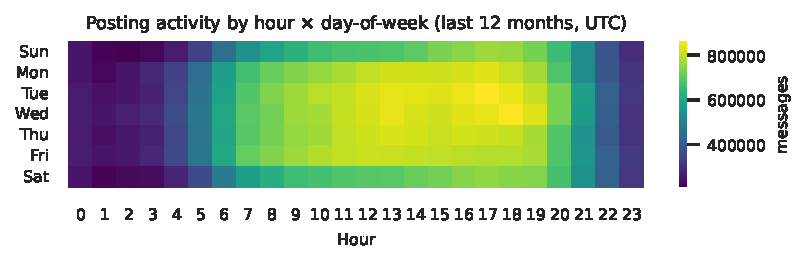
\includegraphics[width=\textwidth]{figures/res_activity_heatmap}
\caption[Posting-activity heatmap.]{Posting activity by hour of day and day of week over the last twelve months (UTC). Activity follows a single daytime cycle peaking in the afternoon and early evening ($14$--$18$\,UTC) and bottoming out overnight; weekend days are modestly quieter than weekdays.}
\label{fig:res-activity-heatmap}
\end{figure}

%======================================================================
\section{Reading the Forward Graph}
\label{sec:res-network}
%======================================================================

The forward references recorded in the corpus reconstruct a directed forward graph. A large fraction of the forwards in that graph are not editorial reposts but automatic copies: when a channel has a linked discussion group, Telegram mirrors each broadcast post into that group as a forward so comments can attach to it. This section removes those copies first, then reports every forward-graph statistic on the cleaned (\emph{editorial}) graph, because the correction has to be in place before any forward-based figure used elsewhere can be trusted.

\paragraph{Auto-mirror copies inflate the forward ratio.}
These auto-mirror copies are forwards in the data but carry no editorial meaning, and they make the raw forward ratio misleading. Of all messages, $18.3\%$ are flagged as forwarded (the raw forward ratio), but $34.0\%$ of those flagged forwards are auto-mirror duplicates; removing them yields an \emph{editorial} forward ratio of $12.1\%$, a $-6.2$ percentage-point correction (Table~\ref{tab:res-fwd-ratio}). Any ``what fraction of Telegram is reposted content'' figure taken from the raw flag therefore overstates editorial reposting by about a third. Every forward-graph result below is computed on the editorial graph, with auto-mirror edges removed.

\begin{table}[htbp]
\centering
\caption[Auto-mirror-corrected forward ratio.]{The forward ratio before and after removing auto-mirror duplicates (a channel's posts copied into its own linked group). Editorial reposting is $12.1\%$ of messages, not the $18.3\%$ the raw flag suggests.}
\label{tab:res-fwd-ratio}
\small
\begin{tabular}{@{}lr@{}}
\toprule
\textbf{Metric} & \textbf{Value} \\
\midrule
Raw forward ratio (\texttt{is\_forwarded} / all messages) & $18.3\%$ \\
Auto-mirror duplicates as share of all flagged forwards   & $34.0\%$ \\
Editorial forward ratio (auto-mirror removed)             & $12.1\%$ \\
Correction                                                & $-6.2$\,pt \\
\bottomrule
\end{tabular}
\end{table}

Removing auto-mirror does more than move the ratio: it changes what the graph looks like. The mirror edges are few but heavy, just $3{,}752$ \mbox{(parent~$\rightarrow$~own-group)} edges, barely a tenth of a percent of the graph, carry about $36\%$ of all forward weight, so on the full graph the largest forwarding community and the top hubs are discussion groups, an artefact of those edges; on the editorial graph ($401{,}928$ nodes, $2.9$\,M edges) the top communities and hubs are broadcast channels, as they should be. The editorial graph is a single giant weakly connected component, and reciprocal forwarding is negligible (the largest strongly connected component is $1.6\%$ of nodes), so forwarding is overwhelmingly one-directional: a small set of source channels feed a large set of repackagers.

\paragraph{Repost networks, not virality.}
Telegram rewrites forward metadata to point at the original sender along the whole chain, so recursive walks over \texttt{fwd\_\allowbreak from\_\allowbreak channel\_\allowbreak id} structurally bottom out at depth~one. The most-forwarded source message in the corpus accumulated $1{,}570$ in-corpus forwards from only four distinct channels, all at depth~one. ``Most-forwarded'' rankings therefore surface dense repost clusters, not viral multi-hop diffusion.

\subsection{The Reference Frontier}
\label{sec:res-frontier}

The corpus records a large frontier of channels it has seen referenced but never crawled. Part of the frontier is permanently out of reach. Of $2.28$\,M hyperlinked \texttt{t.me} references, only about $52\%$ are plain queue-able public handles; roughly $14\%$ are invite-only \texttt{+hash} or web-preview links that our scraper's capture group can never resolve, and a further $24.5\%$ are deep links that point at a message inside an already-queued channel (Figure~\ref{fig:res-frontier}). The invite-only share is a hard structural ceiling rather than a backlog. The unreachable set features clusters by theme (Russian-military and geopolitics discussion, German far-right, Iranian news) and includes the uncrawled discussion groups of major channels such as Kinopoisk, Kommersant, and Khamenei-affiliated news.

\begin{figure}[htbp]
\centering
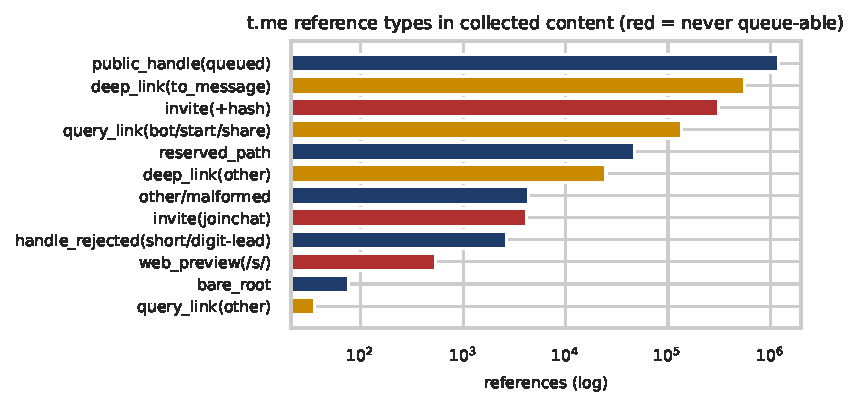
\includegraphics[width=\textwidth]{figures/res_frontier_link_types}
\caption[Frontier link-type breakdown.]{Breakdown of cited \texttt{t.me} references by link type. About half are queue-able public handles; invite-only and web-preview links (roughly $14\%$) are a hard structural ceiling, and deep links (about $24.5\%$) point into already-queued channels.}
\label{fig:res-frontier}
\end{figure}

%======================================================================
\section{Combined Capability Layers}
\label{sec:res-layers}
%======================================================================

This section presents the capabilities that justify the dataset, each traced to the collection mechanism that produced it. The first three subsections cover comments, edits, and deletions; the edit and deletion layers are collected by no prior general-purpose Telegram corpus, and the comment layer only by the concurrent TeraGram~\cite{teragram2026} (and there as a single static snapshot, without the edit and deletion history we pair with it); the fourth covers per-platform restriction, present but unexposed inside serialized message objects in prior corpora and surfaced and analysed here at scale; the fifth gathers in the supporting content surface; the sixth records what we deliberately did \emph{not} find.

\subsection{Comments and Discussion}
\label{sec:res-comments}

A comment is not a first-class object on Telegram. When a broadcast channel turns comments on, the platform attaches a linked discussion group and mirrors every post into it as a byte-identical copy that the channel itself posts (an auto-forward); the comment thread a reader sees is just the set of replies to that mirrored copy. The scraper collects this layer by following the parent's linked-group pointer, registering the group as a \texttt{linked\_group} child with a back-pointer to its parent, and scraping it inline within the same per-channel turn rather than as a separate queue entry (Section~\ref{sec:scraping-cycle}). That design is what turns ``comments'' from an unreachable interface affordance into stored, queryable rows, and it is the mechanism behind the single largest additive layer in Table~\ref{tab:res-scalars}: the $333.2$\,M-message discussion side, which among general-purpose corpora only the concurrent TeraGram~\cite{teragram2026} collects by design.

Comments are identified structurally rather than from the raw \texttt{is\_comment} flag, which the scraper hard-codes to \texttt{false} on every row at collection time. The flag is populated only afterward, by a backfill pass (\texttt{tools/set\_is\_comment.py}) that classifies each discussion-group message by how it attaches to the post stream:

\begin{itemize}
\item An \emph{auto-mirror} is the thread head: the byte-identical copy of a parent post that the channel itself auto-forwards into the group, recognised as channel-authored by \texttt{author\_id} equal to the parent.
\item A \emph{comment} is a reply that anchors on an auto-mirror, either directly (its \texttt{reply\_\allowbreak to\_\allowbreak msg\_\allowbreak id} targets the mirror) or through its thread root (\texttt{reply\_\allowbreak to\_\allowbreak top\_\allowbreak id}) on a nested reply. These are the only rows the flag marks \texttt{true}.
\item \emph{Everything else} stays \texttt{false}: the auto-mirrors themselves (channel copies, not reader replies), free in-group chat (top-level messages with no reply pointer), and replies that answer another member rather than a post.
\end{itemize}

Because the rule keys on the auto-mirror, a comment whose thread-head mirror was never captured (deleted, or outside the crawled range) is missed, so the backfilled flag is a \emph{lower bound} on comments, the counterpart to the reply-pointer count introduced next, which over-states them.

On that structural definition, comments are a plurality of the corpus: $202.5$\,M messages ($42.6\%$ of all messages) carry a reply pointer, and $198.2$\,M of those ($97.9\%$) sit inside a crawled linked discussion group. The comment layer alone is therefore larger than the entire broadcast side ($141.8$\,M). This is a direct consequence of the depth-first design of Section~\ref{sec:res-corpus}: the deepest channels in the corpus are overwhelmingly discussion groups, so sampling fewer channels far more thoroughly disproportionately fills in the comment side. These reply-bearing messages are the layer's raw extent, but they are an \emph{upper bound} on genuine comments-on-posts, for the reason the next correction makes precise.

A reply pointer only records that a message answers some earlier message; it does not record that the earlier message was a broadcast post. Genuine comments-on-posts anchor, directly or transitively, on the mirrored duplicate of a parent post, and that duplicate is byte-identical to the original in $99.8\%$ of matched cases ($47{,}285$ of $47{,}379$), so anchoring can be checked directly rather than assumed. (These mirrored duplicates are exactly the auto-mirror forwards whose contamination of the forward graph Section~\ref{sec:res-network} removes: the thread head a comment replies to is the same edge that inflates the raw forward ratio.) Checking anchoring per group reveals a sharply bimodal population (Figure~\ref{fig:res-anchoring}): the median discussion group anchors $79.4\%$ of its replies on a post, behaving as a true comment section, while a handful of very high-volume chat-style groups reply mostly to one another and drag the reply-weighted pooled anchoring rate down to $58.2\%$. The reply-pointer count therefore over-states comments-on-posts by roughly $42\%$ corpus-wide (about $21\%$ for the median group), and the de-biased comments-on-posts estimate is near $58\%$ of the $198.2$\,M reply-bearing total. The separation of a post-anchored comment section from free in-group chat is itself a finding the discussion-group side cannot be read without. Table~\ref{tab:res-comment-decomp} sets out the resulting decomposition of the whole discussion side, separating the mirrored posts themselves, the comment threads anchored on them, and the in-group messages that carry no mirrored-post reference.

\begin{figure}[htbp]
\centering
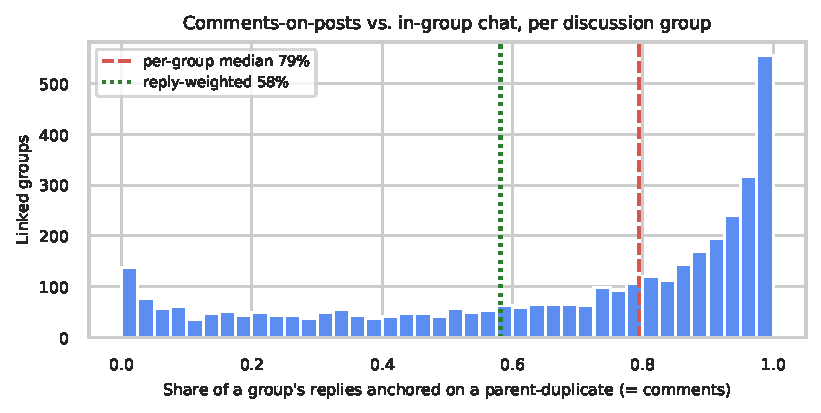
\includegraphics[width=\textwidth]{figures/res_anchoring_rate_dist}
\caption[Comment anchoring-rate distribution.]{Per-group anchoring rate: the share of a discussion group's replies that attach to a mirrored broadcast post rather than to other in-group chat. The distribution is bimodal. Most groups behave as true comment sections (median $79.4\%$), while a few high-volume chat-style groups anchor little and pull the reply-weighted pooled rate down to $58.2\%$, which is why the raw reply-pointer count over-states comments-on-posts.}
\label{fig:res-anchoring}
\end{figure}

\begin{table}[htbp]
\centering
\caption[Decomposition of the linked-group discussion side.]{Decomposition of the $333.2$\,M-message linked-group discussion side into mutually exclusive populations. A member manually forwarding a parent post into the group looks identical on the \texttt{fwd\_from} fields but is sent by a user, so the $0.15$\,M such forwards ($0.5\%$ of matching \texttt{fwd\_from} rows) are counted as standalone messages, not mirrors. \emph{Comments on a mirror} are the replies that anchor, directly or transitively, on a mirrored post, that is, the comment threads of Figure~\ref{fig:res-anchoring}; the next row holds reply-bearing messages that anchor on something else (in-group conversation), and the last holds non-reply group messages. The final two rows together ($188.5$\,M) are the messages with no mirrored-post reference.}
\label{tab:res-comment-decomp}
\small
\setlength{\tabcolsep}{6pt}
\begin{tabular}{@{}lrr@{}}
\toprule
\textbf{Population} & \textbf{Messages} & \textbf{Share} \\
\midrule
Mirrored posts (auto-forward thread heads)          & $29.4$\,M  & $8.8\%$  \\
Comments on a mirror (anchored, incl.\ the thread)  & $115.2$\,M & $34.6\%$ \\
In-group messages not anchored to a mirror          & $82.9$\,M  & $24.9\%$ \\
Standalone group messages (no reply, no mirror)     & $105.6$\,M & $31.7\%$ \\
\midrule
Linked-group discussion side (total)                & $333.2$\,M & $100\%$  \\
\bottomrule
\end{tabular}
\end{table}

The broadcast side carries a complementary signal the discussion side cannot: whether comments were enabled for an individual post. Telegram attaches a replies object (stored as \texttt{replies\_count}, Table~\ref{tab:messages}) to a post only when comments are on for it, so on a broadcast that owns a discussion group, \texttt{replies\_count} being \texttt{NULL} marks comments disabled for that post, $0$ marks enabled-but-empty, and $>0$ marks enabled-with-comments. Across the $67.2$\,M non-service posts on channels that own a discussion group, $46.4\%$ are disabled, $36.8\%$ are enabled but drew no comment, and only $16.8\%$ actually carry comments (Table~\ref{tab:res-comment-toggle}). The decomposition separates a genuinely disabled post from one that was open but ignored, a distinction invisible from the group side where both look like a post with no thread. The toggle is also exercised \emph{within} channels rather than set once: many broadcasters carry both enabled and disabled posts (the interior mass of Figure~\ref{fig:res-comment-toggle}) instead of sitting at all-off or all-on. A capture cross-check corroborates the reading: posts marked enabled carry a matching mirrored duplicate in the linked group $61.4\%$ of the time against only $28.9\%$ for disabled posts, the expected direction, with the residual gap attributable to imperfect chat capture rather than to noise in the signal. What the field cannot show is why or when a post's comments were toggled, because only the latest \texttt{replies\_count} snapshot is stored, with no history.

\begin{table}[htbp]
\centering
\caption[Per-post comment toggle.]{Per-post comment state on the $67.2$\,M non-service broadcast posts belonging to channels that own a discussion group, read from \texttt{replies\_count}. Most posts have comments disabled or enabled-but-empty; only about one in six actually draws a comment. Because the state is read per post, it captures within-channel toggling that the discussion-group side cannot see.}
\label{tab:res-comment-toggle}
\small
\setlength{\tabcolsep}{6pt}
\begin{tabular}{@{}lrr@{}}
\toprule
\textbf{Per-post state} & \textbf{Posts} & \textbf{Share} \\
\midrule
Comments disabled (\texttt{replies\_count} NULL) & $31.2$\,M & $46.4\%$ \\
Enabled, no comments ($=0$)                       & $24.7$\,M & $36.8\%$ \\
Enabled, with comments ($>0$)                     & $11.3$\,M & $16.8\%$ \\
\bottomrule
\end{tabular}
\end{table}

\begin{figure}[htbp]
\centering
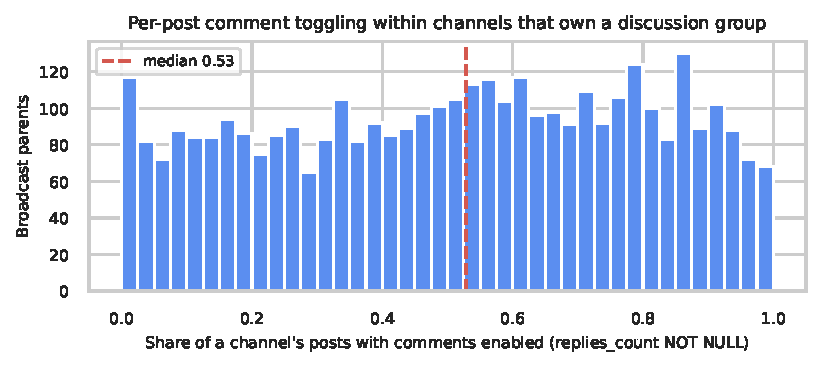
\includegraphics[width=\textwidth]{figures/res_comment_post_toggle}
\caption[Per-post comment toggling within channels.]{Distribution of broadcast channels by the fraction of their posts that have comments enabled. The interior mass shows that toggling is exercised per post within a channel rather than set once; the spikes at $0$ and $1$ are channels that run a single all-off or all-on policy.}
\label{fig:res-comment-toggle}
\end{figure}

Thread shape is best shown on one worked example. The Cycling Market channel and its linked chat hold $391$\,K broadcast posts against $999$\,K discussion messages, a commentariat roughly $2.6\times$ the size of the broadcast stream. Reconstructing reply trees over the chat gives the depth distribution of Figure~\ref{fig:res-thread-depth}: most comments are depth-one replies directly to the post, with a long tail of deeper back-and-forth. The commentariat is heavily concentrated, the two most active accounts alone contributing $18.4\%$ and $17.5\%$ of all human comments, and returning commenters outnumber first-time ones in every month after the section's launch. These thread-structure figures illustrate one active comment section rather than the whole corpus, but they show the granularity the layer supports (per-account, per-thread, and longitudinal), and the moderation behaviour of this layer (comments are deleted about four times as often as posts) is taken up in Section~\ref{sec:res-deletion}.

\begin{figure}[htbp]
\centering
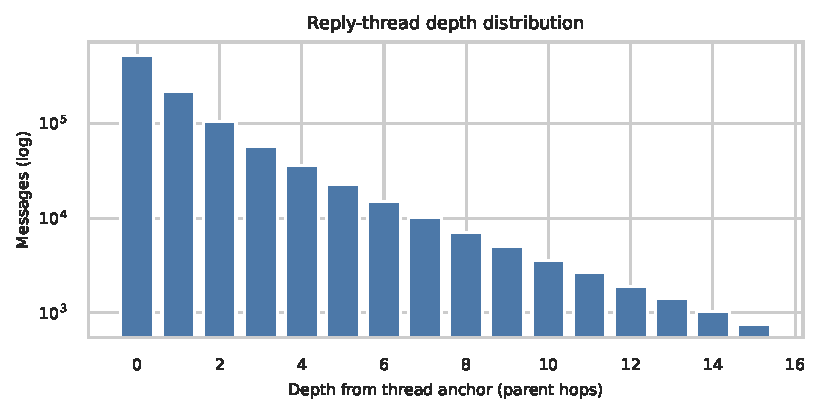
\includegraphics[width=\textwidth]{figures/res_thread_depth_dist}
\caption[Comment thread depth.]{Reply-tree depth distribution for one worked comment section (Cycling Market). Most comments sit at depth one, direct replies to the post; a long tail of deeper threads reflects back-and-forth between commenters.}
\label{fig:res-thread-depth}
\end{figure}

\subsection{Edits: What They Actually Do}
\label{sec:res-edits}

The before/after text of edited messages is a capability no flag-only corpus has, and it overturns the natural proxy for editing. Telegram's permanent \texttt{edit\_date} flag is set on roughly one third of all messages, but it is not a human-edit signal: about $20\%$ of flagged edits land within ten seconds of posting, and roughly three quarters of those are Telegram auto-finalising media albums and link previews rather than a person changing anything (Figure~\ref{fig:res-edit-auto}). Text-only edits, by contrast, skew late.

The diffable archive, the $36{,}016$ edits for which the scraper caught both versions, settles what editing actually does. Of these, $93\%$ leave the message text byte-identical, with the change confined to media, markup, or message entities; the $7\%$ that do rewrite text come to $2{,}356$ before/after pairs, which Claude Sonnet~4.6~\cite{claudesonnet2026} labels against a fixed taxonomy; grouping those labels splits the set $62\%$ substantive editorial against $38\%$ non-substantive. For each pair the model is given the archived before-text and the current after-text and asked to assign exactly one primary label, the \emph{dominant} kind of change, from a fixed nine-type taxonomy (cosmetic, mechanical-counter, factual correction, addition, removal, tone rewrite, compliance annotation, multi, and other) and to add a short free-text note naming the concrete change; the prompt instructs it to judge the change rather than the language, since the corpus is multilingual. Two of the nine types (cosmetic fixes and auto-updating tallies such as vote or view counts) are defined as non-substantive, and that boundary is what draws the $62/38$ line. The full labelling prompt is reproduced in Appendix~\ref{app:edit-prompt}. The single largest type is cosmetic typo, spacing, and markup fixes ($36\%$), followed by additions ($23\%$) and removals ($13\%$), with substantive rewrites, factual corrections, and entity swaps making up the remainder (Figure~\ref{fig:res-edit-taxonomy}). Two further properties sharpen what an edit is for. First, editing is essentially \emph{valence-neutral}: scored with the \texttt{textdetox} XLM-R toxicity classifier~\cite{dementieva2024}, $97\%$ of edits move a message's toxicity by at most $0.05$ on a $0$--$1$ scale, so editing is not systematic de/toxification or sentiment-laundering. Second, what substantive edits churn is \emph{facts}, not tone: a number changes in $39\%$ of them, and under a multilingual named-entity tagger~\cite{tedeschi2021} the most-edited entity types are miscellaneous ($24\%$), locations ($12.6\%$), persons ($11.7\%$), and organisations ($10.2\%$), with additions and deletions roughly balanced per type, that is, substitution rather than net accretion. Editing is also concentrated and skews toward large official channels. The contribution here is a measured replacement for a widely misused flag: the raw flag over-counts human editing by roughly an order of magnitude, and the before/after archive supplies the corrected picture, down to what the edits actually rewrite. The edit-detection mechanism is described in Section~\ref{sec:combined-pass}.

\begin{figure}[htbp]
\centering
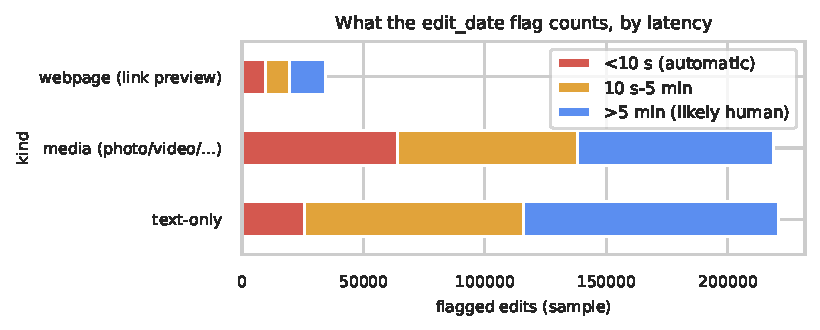
\includegraphics[width=\textwidth]{figures/res_edit_automatic_vs_genuine}
\caption[Automatic vs.\ genuine edits.]{Edits by content kind and time-to-edit. The early spike is dominated by media and link-preview finalisation (automatic), not human editing; text edits arrive later. This is why \texttt{edit\_date} over-counts genuine editing.}
\label{fig:res-edit-auto}
\end{figure}

\begin{figure}[htbp]
\centering
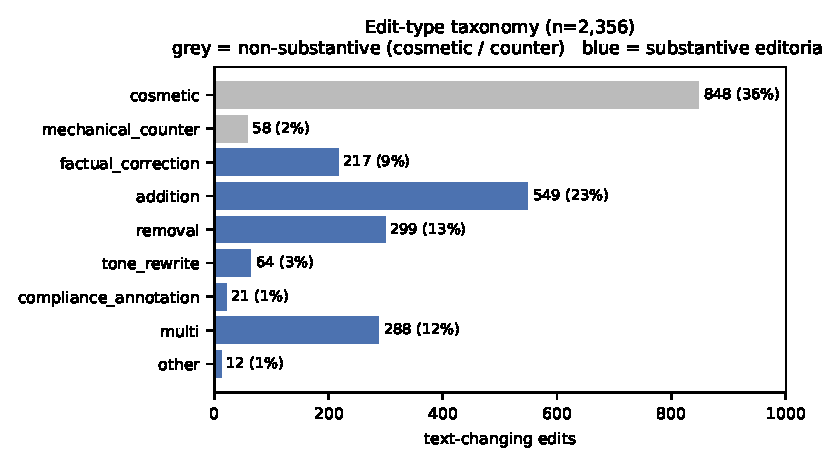
\includegraphics[width=\textwidth]{figures/res_edit_taxonomy}
\caption[Edit-type taxonomy.]{Distribution of the $2{,}356$ text-changing edits across a fixed type taxonomy. A clear majority ($62\%$) are substantive editorial changes (additions, removals, factual corrections, entity swaps) rather than non-substantive ones ($38\%$), of which cosmetic typo and markup fixes are the single largest type at $36\%$.}
\label{fig:res-edit-taxonomy}
\end{figure}

\subsection{Deletion: Thread Purges and Group-Internal Moderation}
\label{sec:res-deletion}

Deletion tracking lets us ask who deletes and whether deletion propagates. Comments are deleted substantially more often than posts: the comment deletion rate is $0.78\%$ against $0.18\%$ for broadcast posts and $0.11\%$ for auto-forward heads (Table~\ref{tab:res-deletion-rates}, Figure~\ref{fig:res-deletion-rates}). Heads are deleted far less than posts, so post deletion is not, in general, sweeping the whole thread away through the mirror copy.

Where deleted comments sit tells a more specific story. Of all deleted comments, $61\%$ sit under a deleted post-thread head, that is, the parent post was itself deleted, so the dominant pattern is thread-level removal: when a post goes, the comments under it go with it (Figure~\ref{fig:res-deletion-root}). The remaining $\sim39\%$ is group-internal: comments removed off a still-alive root ($15\%$), off a deleted native group message ($18\%$), or off a deleted forwarded-in post ($6\%$), reflecting independent moderation and self-deletion inside the group. The capability separates two phenomena the literature tends to conflate: thread-purge deletion driven from the broadcast side, and in-group moderation that the post author never sees.

This split is a property of the collected deleted set, not of deletion on Telegram in general: deletions are detected only on revisit and within a short detection window, so the $2.42$\,M detected deletions are a partial, detection-time sample, and the precise balance between thread-purge and group-internal removal should be read with that sampling in mind. The content of deleted messages is also distinctive. Deleted messages are shorter than surviving ones (median $74$ against $88$ characters) and markedly link-poorer ($4.9\%$ carry a URL against $13.4\%$), and their most over-represented content is spam-token strings and Telegram terms-of-service removal templates rather than any political topic. Deleted content is also more toxic than what survives: against a server-shuffled surviving control, deleted messages score $1.62\times$ higher on the \texttt{textdetox} XLM-R toxicity classifier (mean $0.206$ against $0.128$). That lift is not uniform across the two removal regimes, which target different content: independent in-group moderation, where the parent post survives, removes markedly more-toxic content than a blanket thread-purge that sweeps a whole conversation regardless of content (mean toxicity $0.247$ against $0.187$; Figure~\ref{fig:res-moderation-purge}). Editorial choice targets toxic comments; a thread-purge does not.

Deletion is also concentrated in time: rather than removing content as a steady trickle, a few large discussion groups shed between $100{,}000$ and $320{,}000$ messages in a single day. These spikes are not one phenomenon. Telegram numbers a channel's messages sequentially, so the positions of the deleted ids reveal how a purge was carried out: one long run of consecutive ids means a contiguous block was removed at once, whereas many short runs scattered among surviving ids mean messages were taken out individually. Read this way, the $115$ channels that hold $98\%$ of all purge volume split into three regimes:

\begin{itemize}
\item \textbf{Block-window purges} ($47.3\%$ of the volume): one long contiguous interval, eg. a group clearing its \emph{older} content over a date window while the rest of the channel lives on.
\item \textbf{Scattered moderation} ($35.1\%$): many short intervals interleaved with survivors, eg. a group removing individual comments while the rest of the thread survives.
\item \textbf{Whole-channel wipes} ($17.6\%$): almost the entire channel ($\geq 95\%$) gone in a single detection window.
\end{itemize}

The one-day framing is itself partly an artefact of detection. Because deletions are noticed only on revisit, $87$ of the $115$ channels carry a single detection timestamp: weeks of removals collapse onto the one day the scraper next looked, so a ``purge day'' is a detection event, not necessarily one atomic deletion. The regimes also differ in what they remove. The whole-channel wipes are coherent dead communities taken out wholesale (state-media discussion, anti-vaccine conspiracy, crypto-scam spam), the signature of a channel being taken down or abandoned. The block-window purges instead clear ordinary discussion groups' older content, including 2026 Iran--Israel war chatter, the same event whose two official cohorts the war showcase reads directly for audience toxicity (Section~\ref{sec:res-war}). The deletion-detection mechanism is described in Section~\ref{sec:combined-pass}.

\begin{table}[htbp]
\centering
\caption[Deletion rates by role.]{Detected deletion rate by message role. Comments are deleted about four times as often as broadcast posts; auto-forward heads least of all.}
\label{tab:res-deletion-rates}
\small
\begin{tabular}{@{}lrr@{}}
\toprule
\textbf{Role} & \textbf{Deleted / total} & \textbf{Rate} \\
\midrule
Comment            & $1{,}537{,}202 / 198.2$\,M & $0.78\%$ \\
Broadcast post     & $259{,}617 / 141.8$\,M     & $0.18\%$ \\
Auto-forward head  & $32{,}328 / 29.4$\,M       & $0.11\%$ \\
\bottomrule
\end{tabular}
\end{table}

\begin{figure}[htbp]
\centering
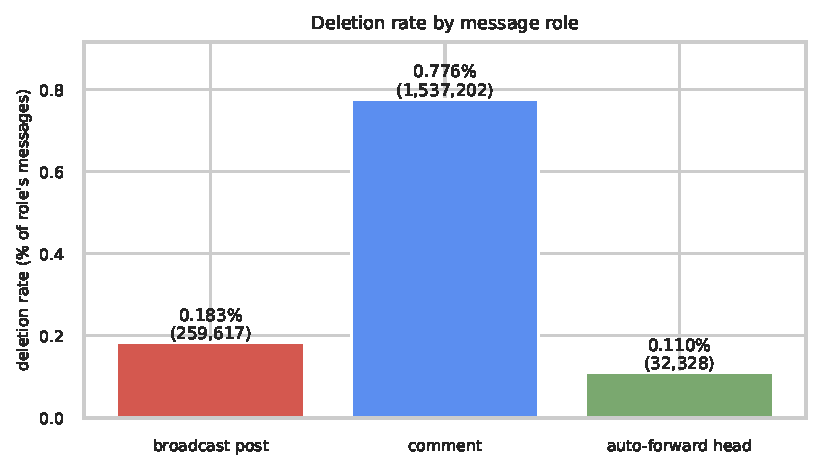
\includegraphics[width=\textwidth]{figures/res_deletion_rates_by_role}
\caption[Deletion rates by role.]{Detected deletion rate by message role. Comments delete more readily than posts; auto-forward heads least, so post deletion does not propagate into the group through the mirror copy at scale.}
\label{fig:res-deletion-rates}
\end{figure}

\begin{figure}[htbp]
\centering
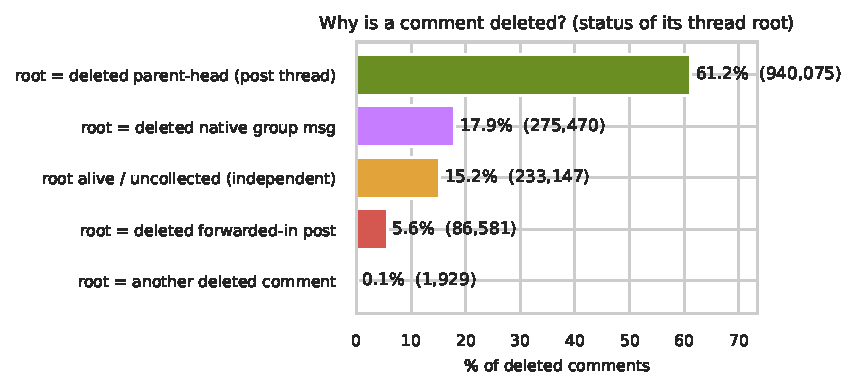
\includegraphics[width=\textwidth]{figures/res_deleted_comment_root_status}
\caption[Deleted-comment root status.]{Where deleted comments sit. A majority ($61\%$) are under a deleted post-thread head (thread-level purge); the remainder are group-internal moderation or self-deletion off still-alive or independently deleted roots.}
\label{fig:res-deletion-root}
\end{figure}

\begin{figure}[htbp]
\centering
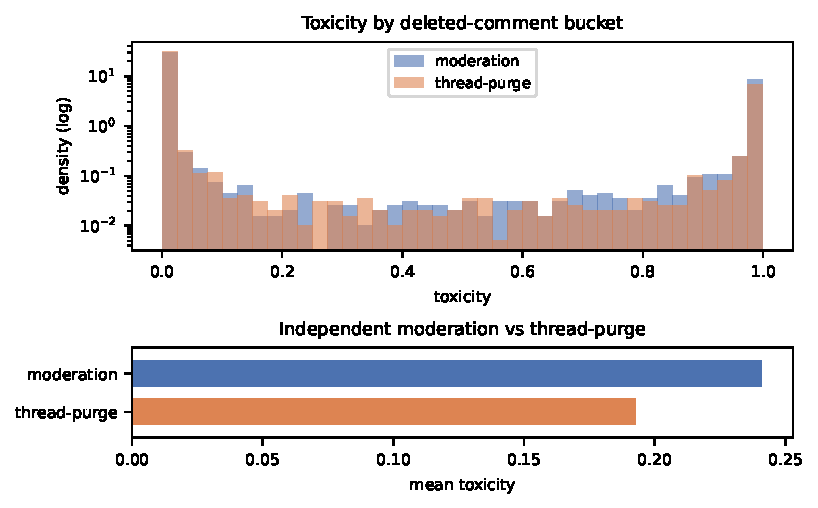
\includegraphics[width=\textwidth]{figures/res_moderation_vs_purge}
\caption[Moderation versus thread-purge toxicity.]{Toxicity of deleted comments split by removal regime. Top: the full toxicity distribution per regime. Bottom: mean toxicity per regime. Independent in-group moderation, where the parent post survives, removes more-toxic content (mean $0.247$) than a blanket thread-purge that removes a whole conversation regardless of content (mean $0.187$), a $1.32\times$ gap. Toxicity scored with the \texttt{textdetox} XLM-R classifier.}
\label{fig:res-moderation-purge}
\end{figure}

\subsection{Restriction and High-Harm Content at Scale}
\label{sec:res-restriction}

The per-platform \texttt{restriction\_reason} flag is a content signal that prior corpora retained only inside serialized message objects and never exposed or analysed; we surface it as a first-class field and study it at scale, a substantial net-new content signal in its own right. $18.7$\,M messages carry at least one restriction flag, indicating content hidden on a specific platform rather than removed (Figures~\ref{fig:res-restriction} and~\ref{fig:res-restriction-platform}, Table~\ref{tab:res-restriction}). The drivers are platform policy, not state censorship: the flags are iOS-heavy, and the largest single content reason is \texttt{porn} ($7.6$\,M flag instances), almost entirely on iOS, reflecting Apple's App~Store rules. A separate and far smaller phenomenon is whole-post obscuring, where Telegram replaces a post's entire content with a service notice that the channel cannot be displayed because it violated the platform's terms of service ($123$\,K such messages in our corpus). This is the form prior work already surfaced: TGDataset reported these obscuring service messages as per-reason counts (its Table~4~\cite{lamorgia2025}). It is also more terminal than per-platform restriction: $13.1\%$ of obscured posts are also deleted, against only $0.8\%$ of restriction-flagged posts. The genuinely net-new signal here is instead the per-platform \texttt{restriction\_reason} field, which prior corpora left untouched; because it is stored as a first-class column (Table~\ref{tab:messages}), these slices are directly queryable.

The same reading holds across language communities once raw counts are normalised (Figures~\ref{fig:res-restriction-lang} and~\ref{fig:res-restriction-lang-rate}). Raw flag instances track representation, English and Russian dominate because they carry the most messages, but the restriction \emph{rate} (flags per $1{,}000$ messages) flips the picture: Russian is among the least restriction-prone communities ($2.3\%$ of messages flagged), while the most restriction-prone are smaller ones, Chinese ($53.8\%$), Polish ($53.1\%$), and Arabic ($49.9\%$), each driven by a single app-store category. Across every language the reasons that survive normalisation are app-store policy categories (\texttt{porn}, \texttt{androidterms}, \texttt{appleterms}, \texttt{appleviolence}), not the Telegram-level \texttt{terms} reason; restriction-proneness varies by community, but the mechanism is App~Store and Play~Store enforcement, not language-specific state censorship. These reason categories also co-occur within the same channels (Figure~\ref{fig:res-restriction-cooccurrence}): a channel hidden under one store category is typically hidden under others, as expected when a single store policy suppresses the same content under several reason codes.

The layer also supports high-harm content slicing, and the behaviour differs sharply by content type. A crypto pump-and-dump cluster deletes at roughly $5.6\times$ the corpus baseline and forwards less, a self-scrubbing pattern, while an extremist cluster barely deletes but forwards more and is comment-heavy, an unrepentant and discussion-driven one. These are rates within our corpus, not absolute prevalence claims.

\begin{table}[htbp]
\centering
\caption[Restriction reasons by flag instances.]{Top per-platform restriction reasons. A message can be flagged on several platforms, so counts are flag instances; the flags are dominated by app-store policy categories, not state moderation.}
\label{tab:res-restriction}
\small
\setlength{\tabcolsep}{6pt}
\begin{tabular}{@{}lrr@{}}
\toprule
\textbf{Reason} & \textbf{Flag instances} & \textbf{Channels} \\
\midrule
\texttt{androidterms}  & $10.57$\,M & $2{,}740$ \\
\texttt{porn}          & $7.63$\,M  & $2{,}402$ \\
\texttt{appleviolence} & $5.05$\,M  & $2{,}194$ \\
\texttt{appleterms}    & $4.27$\,M  & $2{,}402$ \\
\texttt{copyright}     & $0.99$\,M  & $2{,}422$ \\
\texttt{terms}         & $0.19$\,M  & $1{,}815$ \\
\bottomrule
\end{tabular}
\end{table}

\begin{figure}[htbp]
\centering
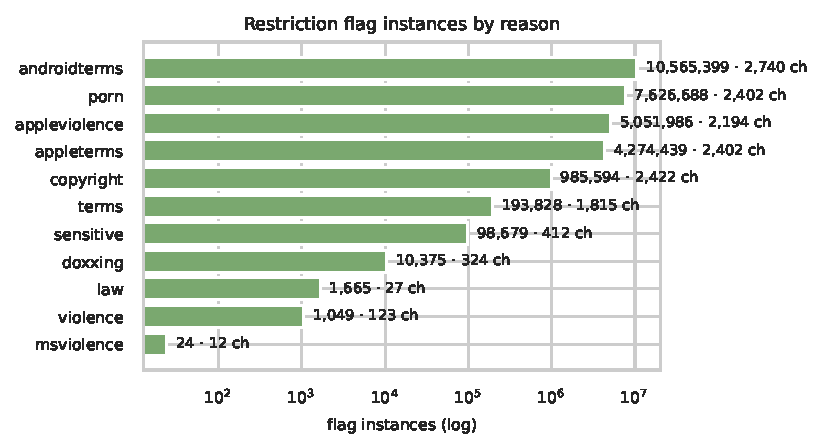
\includegraphics[width=\textwidth]{figures/res_restriction_reasons_by_reason}
\caption[Per-platform restriction by reason.]{Per-platform restriction flag instances grouped by reason, on a $\log_{10}$ scale (flag-instance and channel counts annotated). The flag is dominated by app-store policy categories such as \texttt{androidterms} and \texttt{porn}, indicating store-policy hiding rather than state censorship.}
\label{fig:res-restriction}
\end{figure}

\begin{figure}[htbp]
\centering
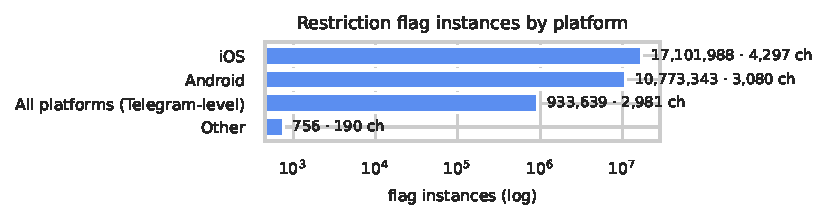
\includegraphics[width=\textwidth]{figures/res_restriction_reasons_by_platform}
\caption[Per-platform restriction by platform.]{The same restriction flag instances grouped by the platform on which the content is hidden, on a $\log_{10}$ scale. Restriction is iOS-heavy, with Android second and a smaller Telegram-level ``all platforms'' share; the opaque minor codes \texttt{VIRT1} and \texttt{ms} (under $10^3$ instances combined) are collapsed into a single \emph{Other} bucket.}
\label{fig:res-restriction-platform}
\end{figure}

\begin{figure}[htbp]
\centering
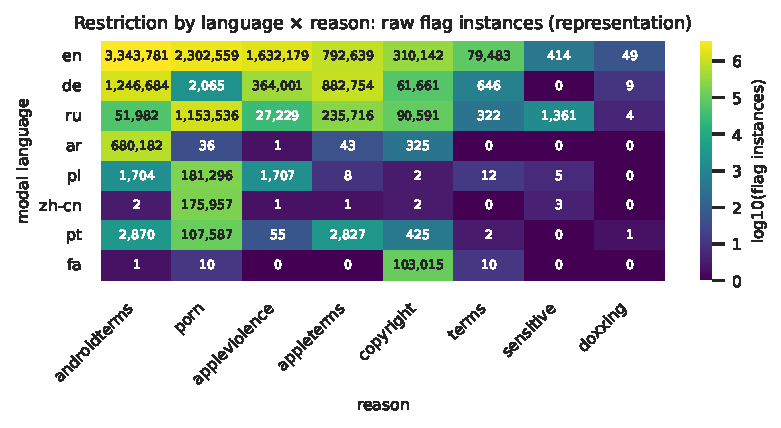
\includegraphics[width=\textwidth]{figures/res_restriction_lang_reason_raw}
\caption[Restriction by language and reason: raw flag instances.]{Restriction by language $\times$ reason, raw flag instances on a $\log_{10}$ colour scale. Raw counts track representation: English and Russian dominate because they carry the most messages, not because those communities are the most restriction-prone (see the normalised view, Figure~\ref{fig:res-restriction-lang-rate}).}
\label{fig:res-restriction-lang}
\end{figure}

\begin{figure}[htbp]
\centering
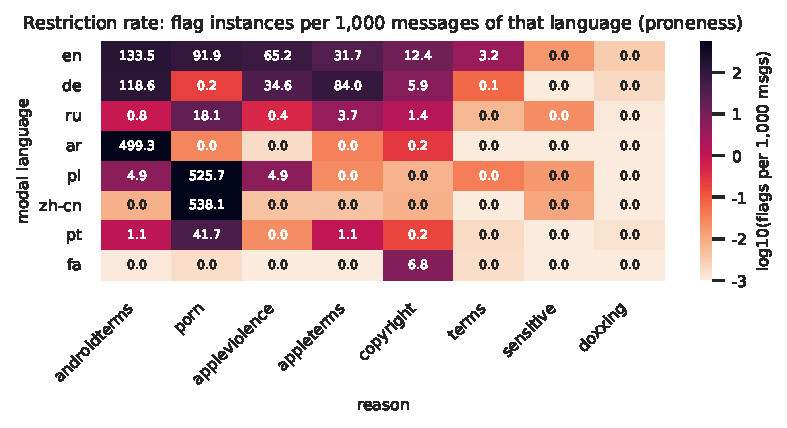
\includegraphics[width=\textwidth]{figures/res_restriction_lang_reason_rate}
\caption[Restriction by language and reason: normalised rate.]{Restriction rate, flag instances per $1{,}000$ messages in each language, on a $\log_{10}$ colour scale. Normalisation isolates restriction-proneness: the communities that survive it (Chinese, Polish, Arabic) are driven by app-store categories (\texttt{porn}, \texttt{androidterms}), not by the Telegram-level \texttt{terms} reason, which is negligible across all languages.}
\label{fig:res-restriction-lang-rate}
\end{figure}

\begin{figure}[htbp]
\centering
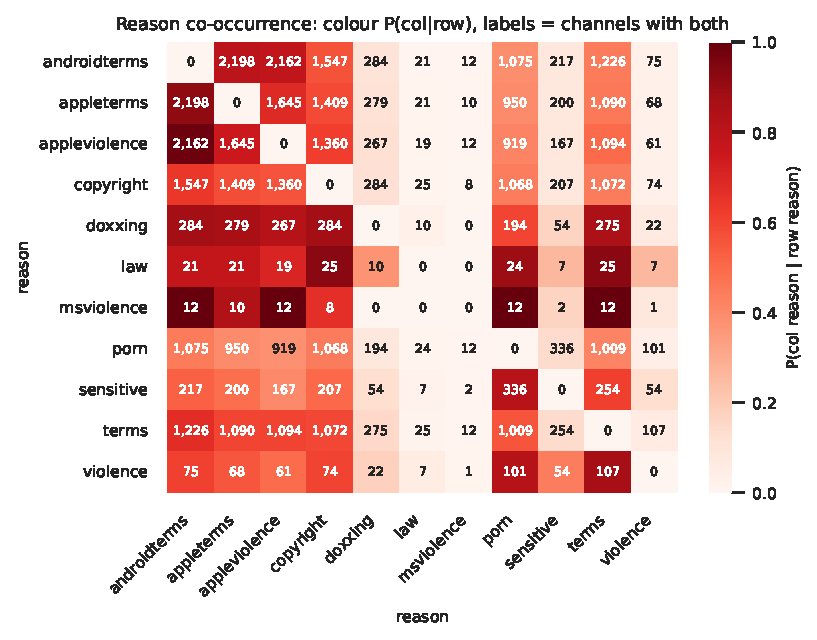
\includegraphics[width=\textwidth]{figures/res_restriction_cooccurrence}
\caption[Restriction reason co-occurrence.]{Co-occurrence of restriction reasons within a channel. Cell colour is the row-conditional share $P(\text{column reason}\mid\text{row reason})$ and the annotation is the number of channels carrying both reasons. The app-store policy categories tend to co-occur within the same channels, consistent with a single store policy hiding the same content under several reason codes rather than reason-specific moderation.}
\label{fig:res-restriction-cooccurrence}
\end{figure}

\subsection{The Content Surface: Engagement, Language, Polls, and Service Actions}
\label{sec:res-content}

The corpus is multilingual, dominated by Russian ($52\%$ of majority-language channels), then English ($18\%$), German ($9\%$), Ukrainian ($5\%$), and Farsi ($5\%$) (Figure~\ref{fig:res-language}); the English share matches TGDataset's $16\%$ almost exactly, while Russian is over-represented relative to it, a composition difference rather than a platform change. Topic shares from a BERTopic model~\cite{grootendorst2022} over the English-language channels are shown in Figure~\ref{fig:res-topics}, led by political news, then COVID and vaccine content, then religion. The language boundary is also a forwarding boundary: channels keep almost all of their forwards in-language (Farsi $99.7\%$, Russian $98.0\%$, German $95.7\%$, English $90.0\%$ of each language's outbound forwards stay same-language), and the dominant language of a linked discussion group matches its parent channel's in nearly every pair. The main exceptions are a modest English--German exchange (about $3$--$5\%$ of forwards each way) and a Russian--Ukrainian bilingual zone, where Ukrainian channels route roughly $15\%$ of their forwards to Russian-language sources and which accounts for almost all of the few group-to-parent language mismatches.

The structured reaction surface supports a genuine but correlational observation: in the most-negatively-reacted-to decile of channels the verified rate is roughly twice that of the most-positive decile ($7.1\%$ against $3.3\%$), and those channels are also several times larger by subscriber count, so the blue check tracks prominence and controversy rather than vetted safety (Figure~\ref{fig:res-verified}). The polls layer ($323$\,K polls) makes both turnout and vote-distribution shape analysable: turnout (voters per view) is recorded for almost every poll and runs at a median of $0.255$, while the $27{,}567$ polls that also store per-option tallies expose the full vote distribution (Figure~\ref{fig:res-polls}); Arabic and Farsi polls stand out as both larger and better attended (median turnout $0.35$ and about $2{,}500$ voters) than the Cyrillic majority (median turnout $0.24$, about $590$ voters). The service-action stream separately records pinning, chat-to-supergroup migrations, and gift and boost adoption (Figure~\ref{fig:res-service}). One language-cohort result deserves a forward pointer: the Farsi cohort is notably ban-resilient, with $99\%$ of channels active before Iran's 2018 Telegram ban~\cite{iranban2018} still active afterward and most still active in 2026. We develop it in the war showcase.

\begin{figure}[htbp]
\centering
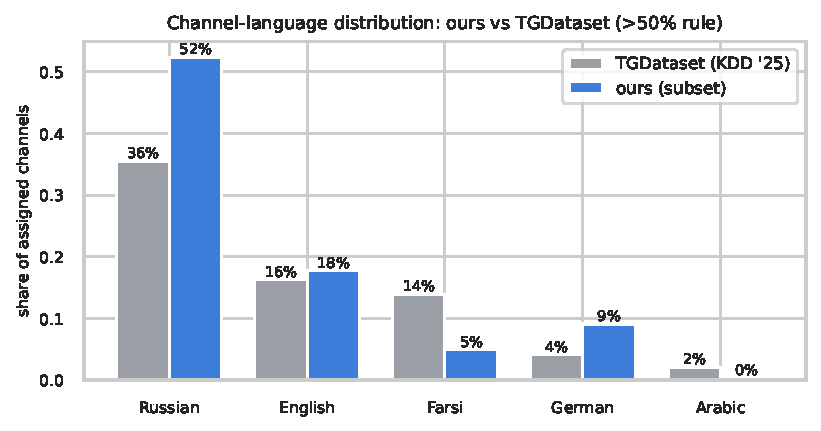
\includegraphics[width=\textwidth]{figures/res_language_distribution}
\caption[Channel language distribution.]{Majority-language distribution across channels with a detected dominant language. Russian dominates, followed by English, German, Ukrainian, and Farsi.}
\label{fig:res-language}
\end{figure}

\begin{figure}[htbp]
\centering
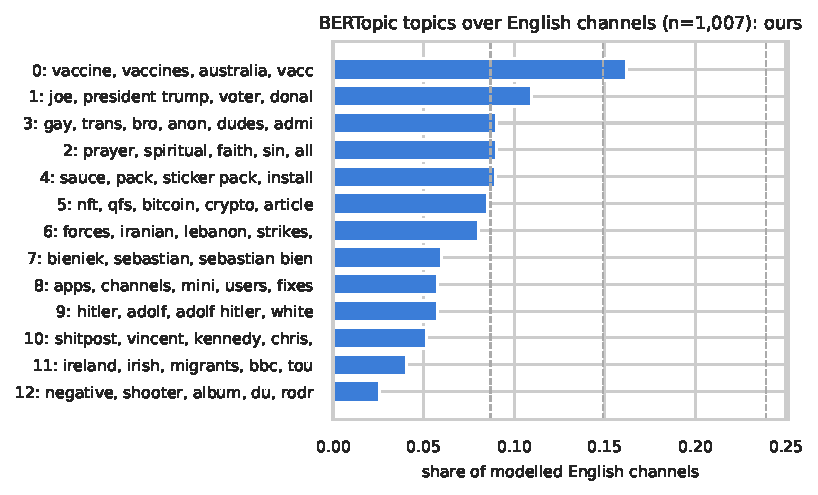
\includegraphics[width=\textwidth]{figures/res_topic_shares}
\caption[Topic shares.]{Channel topic shares from a BERTopic model~\cite{grootendorst2022} over English-language channel content.}
\label{fig:res-topics}
\end{figure}

\begin{figure}[htbp]
\centering
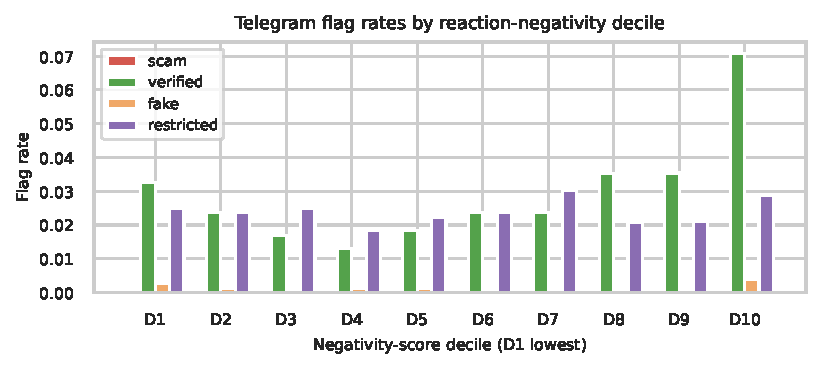
\includegraphics[width=\textwidth]{figures/res_reaction_negativity_flag_rates}
\caption[Verified rate across reaction-negativity deciles.]{Channel flag rates across deciles of audience reaction negativity. The verified rate roughly doubles from the most-positive to the most-negative decile: verification tracks prominence and controversy, not vetted safety.}
\label{fig:res-verified}
\end{figure}

\begin{figure}[htbp]
\centering
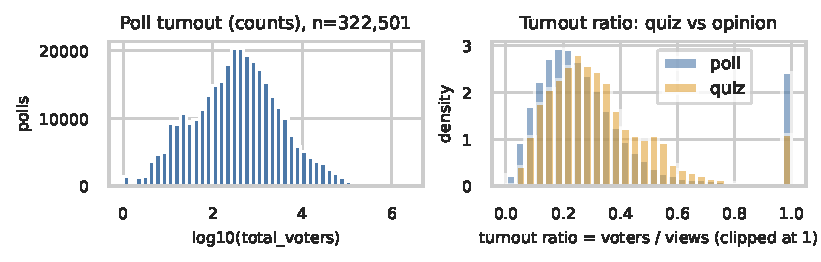
\includegraphics[width=\textwidth]{figures/res_poll_turnout}
\caption[Poll turnout.]{Poll turnout across the corpus. A subset of polls carries per-option vote tallies, making vote-distribution shape analysable.}
\label{fig:res-polls}
\end{figure}

\begin{figure}[htbp]
\centering
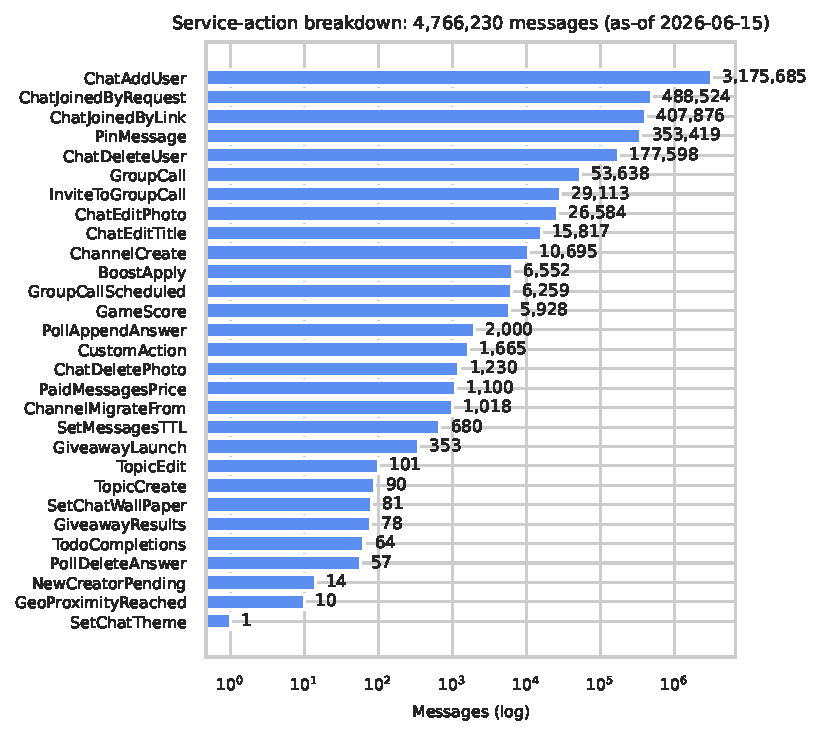
\includegraphics[width=\textwidth]{figures/res_service_actions}
\caption[Service actions.]{Distribution of service actions (pinning, migrations, membership and monetisation events) captured as structured records.}
\label{fig:res-service}
\end{figure}

\subsection{What We Did Not Find, and What to Distrust}
\label{sec:res-nulls}

Two results are valuable precisely as negatives. First, there is no large-scale automated sockpuppet network detectable from profile pictures: across the $12{,}065$ channels scraped for messages, profile images are almost all distinct ($10{,}805$ distinct images), and we find no notable near-duplicate clusters. Second, longitudinal metadata change is tiny: over consecutive-snapshot pairs, only the profile picture ($1.6\%$) and description ($1.2\%$) change appreciably, while the title ($0.3\%$), username ($0.1\%$), and the boolean flags are near zero (Table~\ref{tab:res-metadata}). This is partly a real null and partly a snapshot-density limitation; its concrete value is that it corrected an earlier inflated rate caused by privacy-blanking double-counting.

A final caveat concerns one trust flag that downstream users should treat with caution: \texttt{is\_scam} is set on only five channels and never changes across the snapshot history, so any analysis of scam status over time should rely on \texttt{is\_fake}, \texttt{is\_restricted}, or verification status instead.

\begin{table}[htbp]
\centering
\caption[Consecutive-snapshot metadata change rates.]{Per-pair change rates for channel metadata fields over consecutive snapshots. Only the profile picture and description change appreciably; \texttt{is\_scam} never flips.}
\label{tab:res-metadata}
\small
\setlength{\tabcolsep}{6pt}
\begin{tabular}{@{}lrr@{}}
\toprule
\textbf{Field} & \textbf{Changes / pairs} & \textbf{Rate} \\
\midrule
Profile picture (\texttt{photo\_hash}) & $346 / 21{,}594$ & $1.60\%$ \\
Description                            & $266 / 23{,}116$ & $1.15\%$ \\
Title                                  & $65 / 23{,}116$  & $0.28\%$ \\
Username                               & $14 / 20{,}051$  & $0.07\%$ \\
\texttt{is\_restricted}               & $16 / 23{,}191$  & $0.07\%$ \\
\texttt{is\_scam}                     & $0 / 23{,}191$   & $0.00\%$ \\
\bottomrule
\end{tabular}
\end{table}

%======================================================================
\section{Showcase: USA/Israel--Iran War}
\label{sec:res-war}
%======================================================================

The preceding sections each exercised one capability layer in isolation. A single current event exercises several at once, and the 2026 USA/Israel--Iran war (opening strike $28$~February~2026) is the showcase. The analysis draws on two curated companion databases held alongside the main corpus, \texttt{tgdataset\_iran} and \texttt{tgdataset\_israel}, each built mainly from official and semi-official sources. Each is a bounded crawl: it scrapes a set of official seed channels, their linked comment groups, and the channels they forward from at one hop, and goes no further. The official cohort the figures below rest on is the scraped seeds, $20$ of $27$ on the Iranian side and $25$ of $42$ on the Israeli; counting the comment groups and first-degree forwards as well, the two crawls cover $493$ and $416$ scraped channels respectively (Iran $20$ seeds, $95$ comment groups, $378$ forwards; Israel $25$, $123$, $268$). On the Iranian side these are state news agencies (IRNA, Fars, Mehr, ISNA) together with government and IRGC-affiliated outlets (Press~TV, Tehran~Times, the Khamenei channel); on the Israeli side the IDF, the Home Front Command, the police, government ministries, the emergency services MDA and United~Hatzalah, and the major national outlets. Two commitments run through everything below. Every result is a shift measured against each side's own pre-war baseline (November~2025 to February~2026).

\paragraph{Why Iran is a useful case.}
Section~\ref{sec:res-content} flagged the Farsi cohort as notably ban-resilient: Telegram has remained a usable Iranian information channel through the state's 2018 attempt to block it, with $99\%$ of channels active before the ban still active afterward and most still active in 2026. The wartime data bears this out from the other direction, the Farsi cohort staying near $0\%$ restricted across every restriction reason while the fighting was hottest (Section~\ref{sec:res-restriction}). A surface the state cannot easily suppress is exactly where an official wire is worth watching, which is why the Iranian side anchors the comparison.

\paragraph{The ``flat Iran'' artefact, corrected.}
The snowball reading of the Iranian side, taken from language cohorts in the main corpus, looked flat: pooled daily Farsi volume rose only $1.17\times$ over its pre-war level, the median Farsi channel posted about $0.1\times$ (a net decline), and roughly $30\%$ of channels went silent. Read like for like against the curated Israeli cohort, that picture reverses. The official Iranian wire surged $2.05\times$ over its own pre-war baseline, and the surge is broad-based: the median official Iranian channel more than doubled its output ($2.23\times$), none went silent, and $95\%$ posted more. The Israeli official surface lifts comparably ($2.94\times$ pooled, median $1.78\times$, none silent, $90.9\%$ up). The methodological point is the headline. Snowball sampling, by mixing mostly-dormant grassroots channels into the Farsi cohort, masked a real and broad official mobilisation that only a like-for-like curated comparison recovers (Figures~\ref{fig:res-war-volume} and~\ref{fig:res-war-concentration}).

\begin{figure}[htbp]
\centering
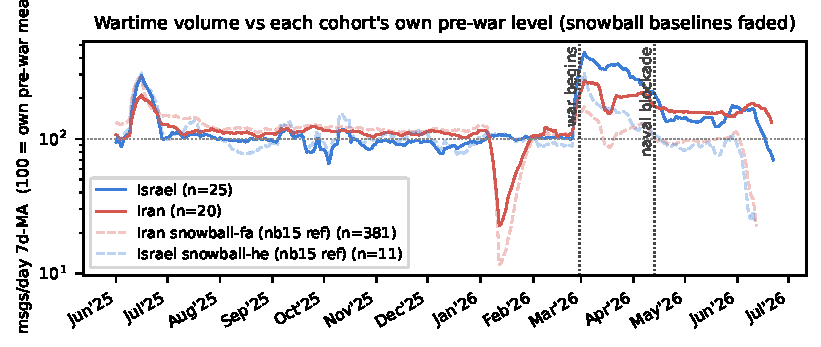
\includegraphics[width=\textwidth]{figures/res_official_volume_index}
\caption[Two official wartime surfaces.]{Daily message volume for the two official cohorts, each indexed to $100$ at its own pre-war (November~2025 to February~2026) mean, with the snowball Farsi and Hebrew language cohorts overlaid faded as the earlier baselines. Both official wires surge over their own pre-war level (Israel $2.94\times$, Iran $2.05\times$); the snowball Farsi line ($1.17\times$) is the flat reading the curated comparison reverses.}
\label{fig:res-war-volume}
\end{figure}

\begin{figure}[htbp]
\centering
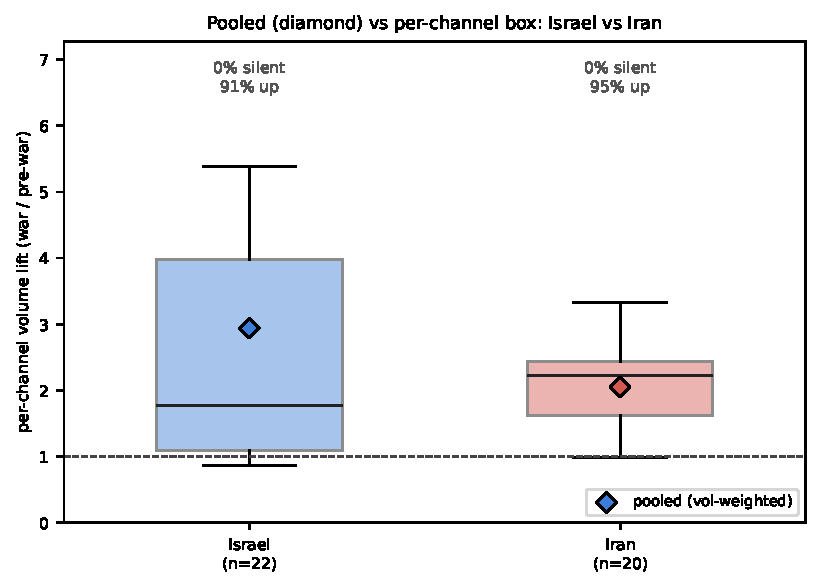
\includegraphics[width=\textwidth]{figures/res_per_channel_lift}
\caption[Pooled versus typical official channel.]{Per-channel war-versus-pre volume lift for each official cohort: pooled lift (diamond) against the channel-level distribution (box). On both cohorts the median channel more than doubled (Iran $2.23\times$, Israel $1.78\times$) with none falling silent, the opposite of the snowball Farsi cohort's median $\sim0.1\times$ and $\sim30\%$ silent. The broad official mobilisation is not a loud-minority effect.}
\label{fig:res-war-concentration}
\end{figure}

\paragraph{Where the surge comes from.}
Splitting each cohort's volume into an extensive margin (how many channels are active) and an intensive margin (how much each active channel posts) locates the surge. Neither official cohort loses channels at the opening strike: the active-channel step is $1.17\times$ for Israel and $0.99\times$ for Iran. Both instead ramp on the intensive margin (Israel $3.76\times$, Iran $2.45\times$), the same channels simply posting far more. This is the opposite of the snowball Farsi cohort, whose active-channel count roughly halved at the opening strike ($0.56\times$): the apparent collapse in the snowball reading was its dormant grassroots tail going quiet, not the official wire contracting.

\paragraph{Institution-fixed multilingual escalation.}
The cleanest, selection-free signal holds a single institution fixed and compares its parallel language arms, so any divergence is audience targeting rather than which channels were sampled. The pattern is symmetric across both states: each escalates its English or international arm hardest. The IDF lifts its English arm $5.39\times$ against $3.87\times$ Hebrew and $2.82\times$ Arabic; IRNA lifts English $1.64\times$ against $1.14\times$ Persian; Mehr lifts English $2.46\times$ against $1.90\times$ Persian; and the English-only Tehran~Times rises $47.5\times$ from a near-dormant pre-war base, a figure to read as a direction (an international arm switched on for the war) rather than a precise multiplier. With the institution held fixed, there is no sampling confound left, and the wartime priority on both sides is plainly the international narrative (Figure~\ref{fig:res-war-arms}).

\begin{figure}[htbp]
\centering
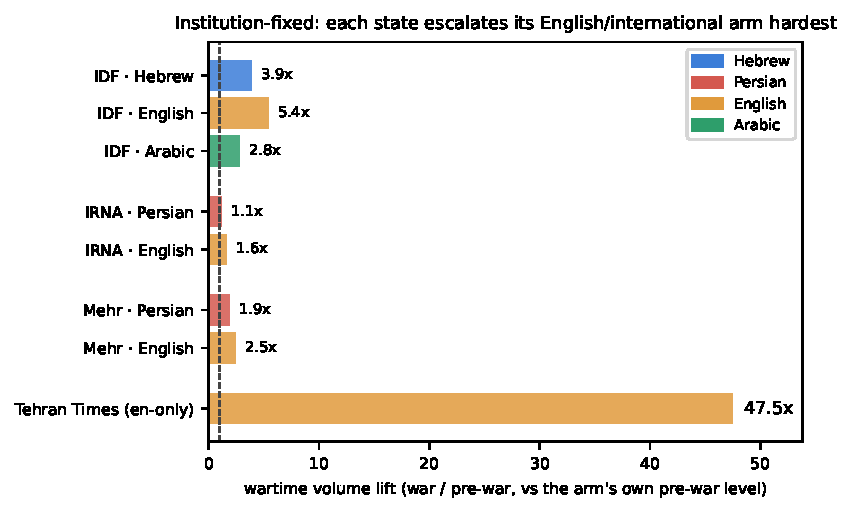
\includegraphics[width=\textwidth]{figures/res_institution_arms}
\caption[English arm escalates hardest, both states.]{War-versus-pre volume lift for the parallel language arms of single institutions (IDF he/en/ar, IRNA and Mehr fa/en, Tehran~Times en-only), each arm indexed to its own pre-war mean. Because the institution is fixed, the divergence is audience targeting, not channel selection: each state escalates its English or international arm hardest.}
\label{fig:res-war-arms}
\end{figure}

\paragraph{Editorial tempo and the air-war clock.}
The war also pushed both wires off their peacetime editorial clock. The share of posting in the local overnight window roughly tripled on each side (Israel $4.0$ to $13.4\%$, Iran $4.5$ to $15.5\%$), as office-hours posting gave way to a more around-the-clock reactive cadence. An exogenous timing signal corroborates the shift: the Israeli Home Front Command's public missile-alert feed, which fired $14{,}122$ alerts over the war window, correlates at $r\approx0.61$ with the daily output of the official Iranian wire (Figure~\ref{fig:res-war-clock}). The two surfaces are keyed to the same air-war clock.

\begin{figure}[htbp]
\centering
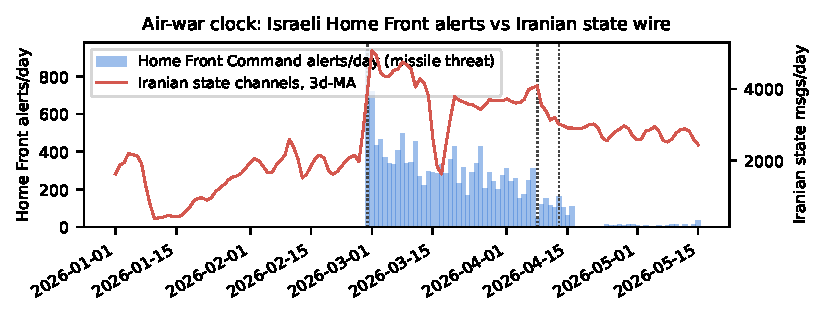
\includegraphics[width=\textwidth]{figures/res_homefront_clock}
\caption[Home Front alerts against the Iranian state wire.]{Daily Israeli Home Front Command missile alerts ($14{,}122$ over the war window) against the daily output of the Iranian state wire. The two track the same exogenous air-war clock ($r\approx0.61$), an external timing reference that neither side controls.}
\label{fig:res-war-clock}
\end{figure}

\paragraph{Audience reaction valence.}
Audience reaction valence, a language-neutral positive-minus-negative score over the structured reaction surface, swung far more on the Iranian side. The Iranian official audience moved from $+0.103$ to $+0.662$ (a shift of $+0.56$ over roughly $2.9$~million wartime reactions), against the Israeli audience's $+0.229$ to $+0.318$ ($+0.09$ over about $0.44$~million). Read as an audience-approval proxy and compared as each side's own shift rather than across sides, the Iranian state audience rallied around its wire far harder than the Israeli audience did around its own.

\paragraph{Narrative convergence and overlap.}
Whether the two surfaces are even covering the same war can be measured directly with cross-lingual sentence embeddings (\texttt{paraphrase-multilingual-MiniLM-L12-v2})~\cite{reimers2019,reimers2020} over each side's domestic-language broadcasts. Daily cross-side centroid cosine similarity is high throughout and peaks at $0.914$ on the $8$~April ceasefire (mean $0.851$ over the $61$-day window): both wires orient to the same exogenous events (Figure~\ref{fig:res-war-framing}). The overlap is asymmetric, though. At a cosine threshold of $0.6$, $95.9\%$ of Iranian broadcasts have an Israeli semantic counterpart, against only $79.3\%$ the other way: the Israeli wire carries more siloed home-front, municipal, and health content with no Iranian analogue, while the Iranian wire maps almost entirely onto the shared war narrative.

\begin{figure}[htbp]
\centering
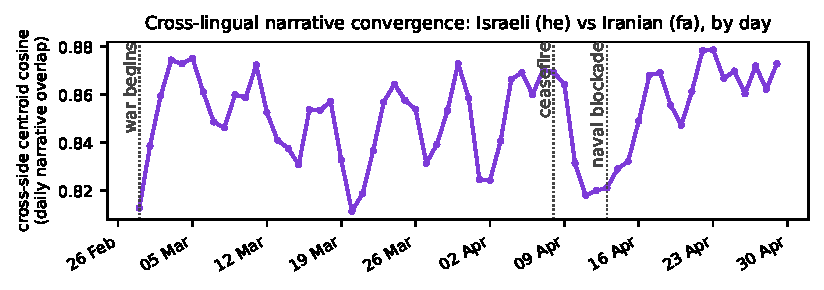
\includegraphics[width=\textwidth]{figures/res_framing_convergence}
\caption[Cross-side narrative convergence.]{Daily cross-side centroid cosine similarity between the two official wires' domestic-language broadcasts, from cross-lingual sentence embeddings. Convergence is high throughout and peaks at $0.914$ on the $8$~April ceasefire (mean $0.851$ over $61$ days): both surfaces orient to the same events. The cosines are approximate; read the temporal shape, not absolute levels.}
\label{fig:res-war-framing}
\end{figure}

\paragraph{Audience toxicity.}
The comment audiences under the two wires also differ in hostility. Scored with the \texttt{textdetox} XLM-R toxicity classifier~\cite{dementieva2024}, the Iranian official comment audience runs $23.4\%$ toxic against the Israeli audience's $18.6\%$. The English-language sections are the nastiest on both sides (around $30\%$ each), and on the Arabic axis, the firmest cross-lingual comparison for this classifier, the Iranian audience ($16.4\%$) again tops the Israeli ($10.8\%$) (Figure~\ref{fig:res-war-toxicity}). These are classifier labels on bounded per-side samples (about $9{,}000$ comments each), so the contrast and its direction carry the reading, not the exact percentages.

\begin{figure}[htbp]
\centering
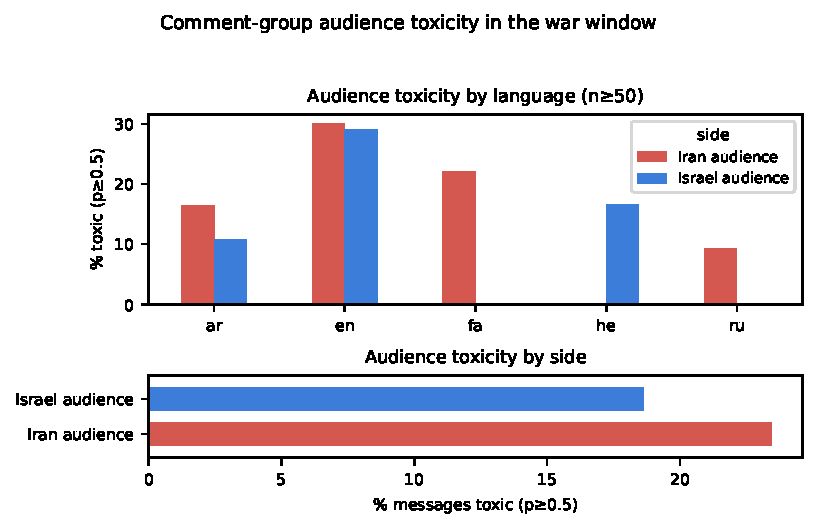
\includegraphics[width=\textwidth]{figures/res_toxicity_by_side}
\caption[Two official audiences' toxicity.]{Toxic-comment share in the two official cohorts' discussion-group audiences, scored with the \texttt{textdetox} XLM-R classifier. Top: by audience language; bottom: by side. The Iranian audience ($23.4\%$) runs more toxic than the Israeli ($18.6\%$); on the Arabic axis (the firmest cross-lingual comparison) the same direction holds ($16.4\%$ against $10.8\%$). Bounded samples of about $9{,}000$ comments per side; read the contrast, not the point values.}
\label{fig:res-war-toxicity}
\end{figure}

\paragraph{Polls and audience composition.}
Two smaller layers round out the showcase. Polls behave as state opinion probes: the official Iranian wire runs them more frequently and to several times the reach of the Israeli wire (median $4{,}310$ voters against $738$), though poll frequency fell on both sides during the war as hard news displaced engagement-polling. And the comment audiences differ in composition: the Iranian official audience is markedly more multilingual (Farsi $52\%$, English $24\%$, Arabic $14\%$) than the Israeli (Hebrew $66\%$, English $25\%$, Arabic $5\%$), consistent with the international-arm escalation seen on the broadcast side.

\paragraph{What the showcase exercises.}
A single event therefore exercises the comment, reaction, poll, language, and (corpus-wide) deletion layers at once, and the analysis is method-led throughout: per-cohort indexing against each side's own baseline, a pooled-versus-median decomposition that overturns the general snowball reading, institution-fixed multilingual contrasts, and an exogenous timing clock. Every figure here is a lead about how two state information surfaces behaved, read against each side's own baseline on small, separately-sampled cohorts in a companion database. The Iranian official cohort in particular is a lower bound: $20$ of $27$ official seeds were captured across the two scrape runs, and the seven missing include heavyweights such as Tasnim and Sepah/IRGC, so its volume and concentration figures understate the full official wire.
